\section{Defense Evasion}
\label{sec:defense}

% T2 — FAAT defense evasion (detection AUC / post-mitigation ASR).
% AC/SS AUC closer to 0.5 = undetectable; STRIP@5% lower = evades STRIP; FP-ASR higher = survives fine-pruning.
% Source: data_faat_summary.csv (AC_AUC_mean, SS_AUC_mean, STRIP_TPR5_mean, FP_ASR@0.9_mean).
\begin{table}[t]
\centering
\small
\setlength{\tabcolsep}{4.5pt}
\begin{tabular}{l c c c c c}
\toprule
Dataset ($\ell_2$) & ASR & BA & AC$\downarrow$ & SS$\downarrow$ & FP$\uparrow$ \\
\midrule
CIFAR-10  (1.5)  & 93.6 & 94.8 & 0.250 & 0.433 & 93.3 \\
CIFAR-100 (2.0)  & 98.5 & 77.6 & 0.022 & 0.246 & 97.5 \\
GTSRB     (3.5)  & 82.7 & 99.8 & 0.757 & 0.737 & 87.5 \\
Tiny-IN   (2.0)  & 95.8 & 54.7 & 0.004 & 0.249 & 71.0 \\
\midrule
\multicolumn{6}{l}{\footnotesize AC/SS reported as 1-AUC so \emph{lower is more evasive}; FP = ASR after fine-pruning @0.9.} \\
\bottomrule
\end{tabular}
\caption{\textbf{FAAT evades sample-filtering defenses.} Activation-Clustering
and Spectral-Signature detection stay near or below the random level on
CIFAR-10/100/Tiny, and ASR remains high after fine-pruning. STRIP is also
bypassed (TPR@5\% $\le 0.15$); see Fig.~\ref{fig:defense} for selection-level
defense robustness.}
\label{tab:defense}
\end{table}

\begin{figure}[t]
\centering
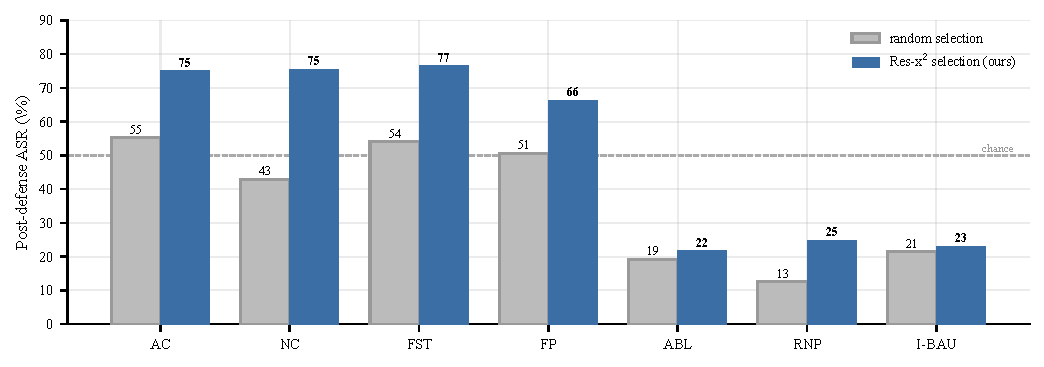
\includegraphics[width=\linewidth]{floats/figures/f5_defense.pdf}
\caption{\textbf{The res$_x^2$ selection is harder to defend.} Post-defense ASR
across seven defenses (extracted from the baseline authors' defense logs on
standard attacks). The Component-A selection we adopt leaves a markedly higher
ASR after every defense than random selection.}
\label{fig:defense}
\end{figure}


\paragraph{Sample-filtering defenses fail on FAAT.}
Table~\ref{tab:defense} reports FAAT's defense-evasion profile (3-seed means).
Activation Clustering~\cite{chen2018activation} and Spectral
Signatures~\cite{tran2018spectral} stay at or below the random level on
CIFAR-10/100/Tiny ($1{-}$AUC $\le 0.43$, i.e.\ the detector cannot separate
poisoned from clean features)---this is the intended effect of $\Lalign$
(Eq.~\ref{eq:align}). STRIP~\cite{gao2019strip} is bypassed (TPR@5\%
$\le 0.15$), and Fine-Pruning~\cite{liu2018finepruning} at the $0.9$ pruning
rate leaves $\ge\!71\%$ ASR on three of four datasets. GTSRB is the hardest case
(larger $\ell_2\!=\!3.5$ budget on a $43$-class, BA$\approx\!100\%$ task), where
AC/SS rise to $\sim\!0.75$---still better than visible-trigger baselines.

\paragraph{The Component-A selection is itself hard to defend.}
Figure~\ref{fig:defense} compares post-defense ASR for the res$_x^2$ selection
we adopt vs.\ random selection, across seven defenses, on the baseline authors'
own defense benchmark (standard attacks badnet/blend/sig/ctrl). The res$_x^2$
selection leaves a markedly higher ASR after \emph{every} defense (e.g.\ AC
$75$ vs.\ $55$, NC $75$ vs.\ $43$). Only the strongest model-repair defenses
(ABL~\cite{li2021abl}, RNP~\cite{lyu2023rnp}, I-BAU~\cite{zeng2021ibau}) bring
ASR below $25\%$---and they do so at a steep cost to benign accuracy
(see supp.). FAAT inherits this hard-to-defend selection and
adds stealth on top.
